\section{System Implementation} \label{system_partitioning}
As briefly discussed in the \textit{Introduction} chapter, nowadays one of the smartest techniques deployed for autonomous vehicles control is the Model Predictive Control, hence our decision to develop a controller in order to accomplish the path following and obstacle avoidance task.
The design of such a controller needs a deep analysis of the project requirements and a smart system partitioning to identify different tasks that can be developed autonomously and independently from others to be then merged in order to satisfy the control problem.


\subsection{Analysis of requirements}
Starting from the detailed system requirements described in Section \ref{System_Requirements}, we can obtain low level requirements suitable for the controller implementation; each of these is associated with a draft of the validation method needed to assert each of them. Table \ref{tab:requirement} shows the system requirements, low level requirements and the corresponding validation methods.

\newcolumntype{P}[1]{>{\raggedright\arraybackslash}p{#1}}
\begin{table}[H]
\begin{tabular}{P{0.33\textwidth} P{0.33\textwidth} P{0.33\textwidth}}
\hline
\multicolumn{1}{c}{\textbf{System requirements}} & \multicolumn{1}{c}{\textbf{Low level requirements}} & \multicolumn{1}{c}{\textbf{Validation methods}} \\ 
\hline
Maximum lateral error from reference of $0.5 m$ & Inequality constraint: $e_{y}=abs(Y_{reference}-Y_{vehicle})<=0.5m$ & Check in each point that the difference between the actual vehicle position and the reference path is not greater than $0.5 m$ \\ 
\hline
Detection of obstacles within 100 m ahead of vehicle & Sensor fusion able to provide useful data in the range $0-100 m$ from the vehicle & Drive toward a static obstacle and confirm that is detected when is $100 m$ far \\ 
\hline
Move on left lane within a predetermined safe zone from the obstacle & Inequality constraint when obstacle detected: $dist = position_{vehicle}-position_{obstacle}  \in Safe Zone$ & Confirm that when changing lane the distance from the obstacle measured by the sensors is greater than the predetermined safe zone \\ 
\hline
Once passed the obstacle, come back on right lane with no less than $10 m$ but no more than $50 m$ ahead of it & Inequality constraint when obstacle passed: $10m <= dist <= 50m $ & Confirm that when changing lane the distance from the obstacle measured by the sensors is greater than the predetermined safe zone \\ 
\hline
Maximum lateral acceleration of $0.5 m/s^2$ & Constraint on Model Predictive Control input: $a.max = 0.5$ & Check that the maximum value registered by the IMU$-$accelerometer is not greater than $0.5m/s^2$ \\ 
\hline
All previous requirements satisfied in speed range from $10 km/h$ to $100 km/h$ & Verify all previous constraint when simulating at speed range $10-100 km/h$ & Verify all the above methods with vehicle travelling from $10 km/h$ to $100 km/h$ \\ 
\hline
\end{tabular}
\caption{System requirements and possible validation methods}
\label{tab:requirement}
\end{table}

\subsection{Partitioning} \label{partitioning_subsection}

Regarding the system partitioning, which as already said in Section \ref{system_partitioning} is a crucial part of the implementation of a system, we have decided to base the implementation of our project on the tasks shown in Figure \ref{fig:partitioning}.

\begin{figure}[H]
    \centering
    \makebox[\textwidth][c]{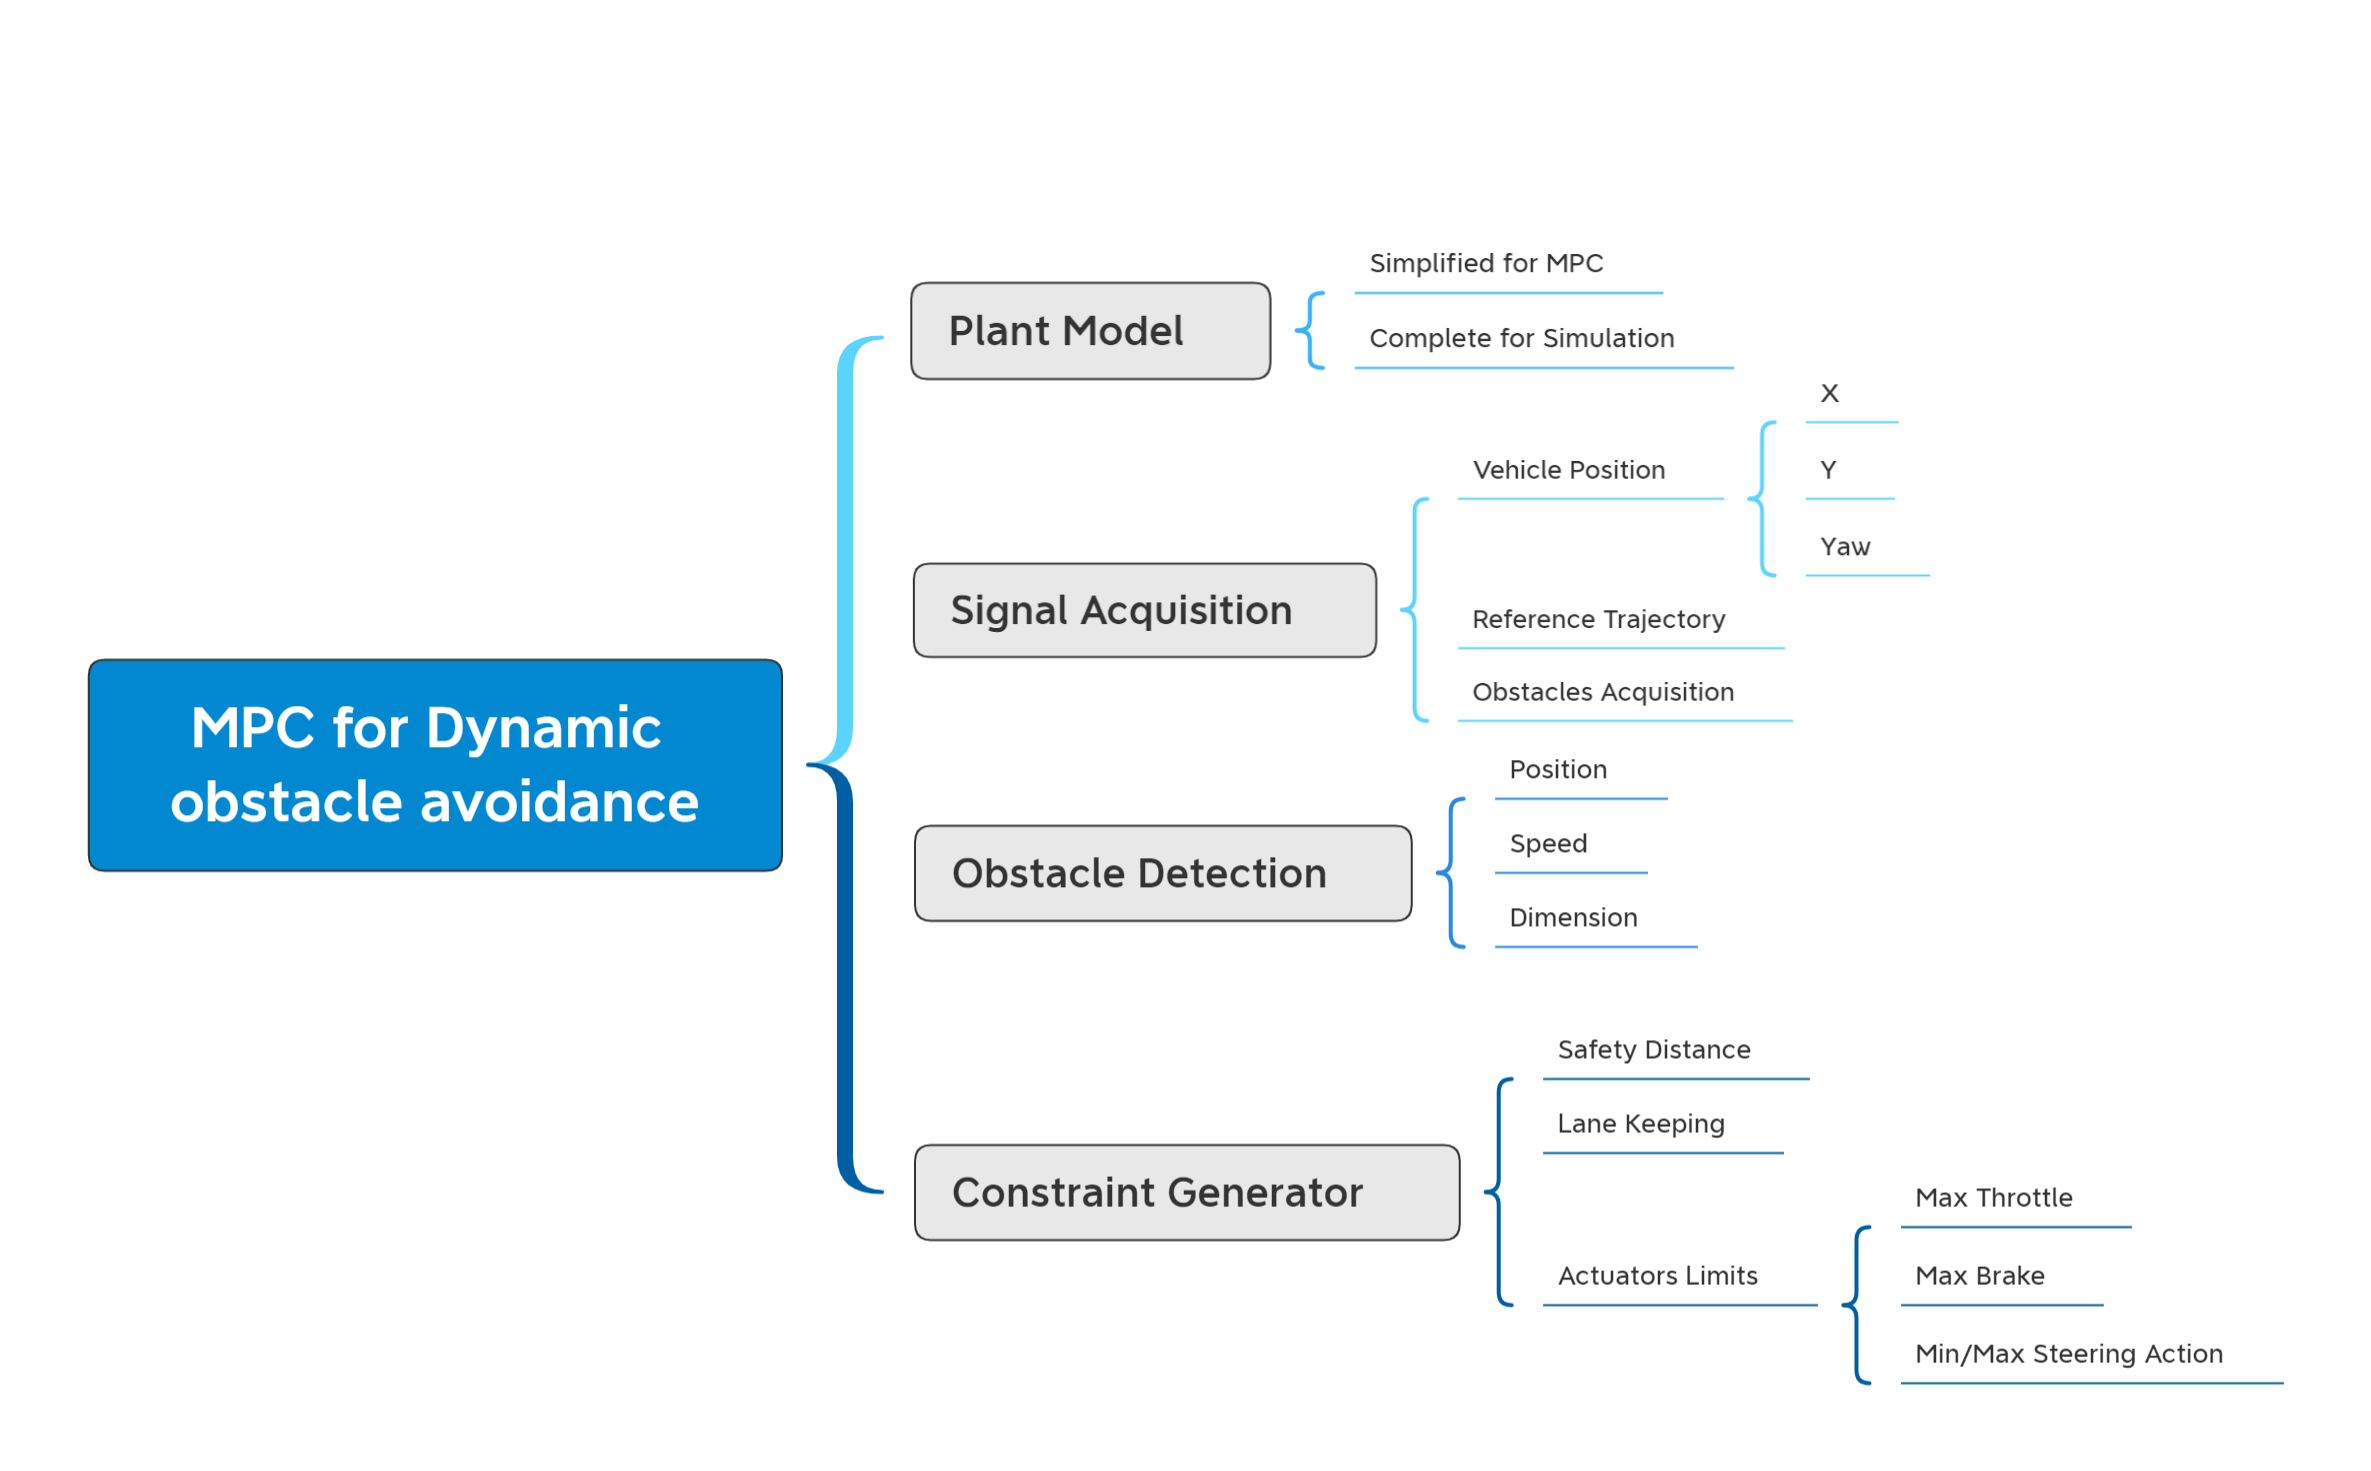
\includegraphics[width=1.25\textwidth,keepaspectratio]{Figures/partitioning.png}}
    \caption{System Partitioning}
    \label{fig:partitioning}
\end{figure}

As shown in the figure above, our project can be divided into four macro-areas:
\begin{itemize}
    \item Plant Model: is the mathematical model of the vehicle which represent the development environment of our project. We have decided to adopt two models, a simplified one to be used in the MPC and a more accurate one to be used in the simulation; 
    \item Signal Acquisition: refers to the gathering of data related to the vehicle position, trajectory, and obstacle acquisition, all coming from the sensors mounted on our vehicle;
    \item Obstacle Detection: here the properties of the obstacle such as position, speed, and dimension  are evaluated;
    \item Constraint Generator: in this phase we set the constraints which the MPC needs to comply with. These constraints are necessary in order to make our model as realistic and safe as possible.
\end{itemize}

These sections will be described in depth in the following chapters.




